\documentclass{standalone}
\usepackage{tikz}
\usepackage{ctex,siunitx}
\setCJKmainfont{Noto Serif CJK SC}
\usepackage{tkz-euclide}
\usepackage{amsmath}
\usetikzlibrary{patterns, calc}
\usetikzlibrary {decorations.pathmorphing, decorations.pathreplacing, decorations.shapes,}
\begin{document}
\small
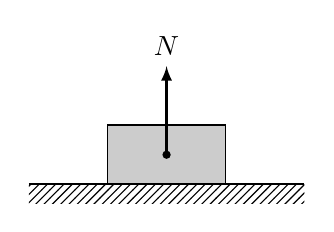
\begin{tikzpicture}[>=latex]
  % \useasboundingbox(-1,-0.75)rectangle(3.7,1.4);
  \draw [fill=black!20,semithick](0,0) rectangle (1.5,.75);
  \fill [pattern = north east lines] (-1,-.25) rectangle (2.5,0);
  \draw [thick](-1,0)--(2.5,0);
  \draw[->,thick](.75,.375)--(.75,1.5)node[above]{$N$};
  \fill (.75,.375) circle[radius=1.5pt];
  \end{tikzpicture}
\end{document}